
%------------------------------------------------

\section{Change of variables}\index{change of variable}
\label{exer:change_of_var}

\subsection{Quadratic}\index{change of variable!quadratic}
\label{exer:change_of_var_quadratic}

\paragraph{Gaussian distribution}\index{Gaussian distribution}

\begin{enumerate}
	\item Take the variables $x$ and $y = x^{2}$.
	\item Assume $x$ is Gaussian distributed with $\mu = 2$ and $\sigma = 1$. (Figure~\ref{fig:change_of_var_Gaussian})
	\item Populate histogram with $10^{6}$ random values of $x$, and a second histogram with the corresponding value of $y$. (Figure~\ref{fig:change_of_var_Gaussian})
	\item Compare the generated distribution of $y$ with the theoretical curve (Figure~\ref{fig:change_of_var_Gaussian_squared}):
		$$
		g(y) = f(x) \left| \frac{\mathrm{d}x}{\mathrm{d}y} \right| 
		= \frac{f(x)}{\left| y'(x) \right|} 
		= \frac{f(x)}{2 \left| x \right|} 
		= \frac{f(-\sqrt{y})}{2 \left| -\sqrt{y} \right|} + \frac{f(\sqrt{y})}{2 \left| \sqrt{y} \right|} 
		= \frac{f(-\sqrt{y}) + f(\sqrt{y})}{2 \sqrt{y}}
		$$
\end{enumerate}

\begin{figure}
	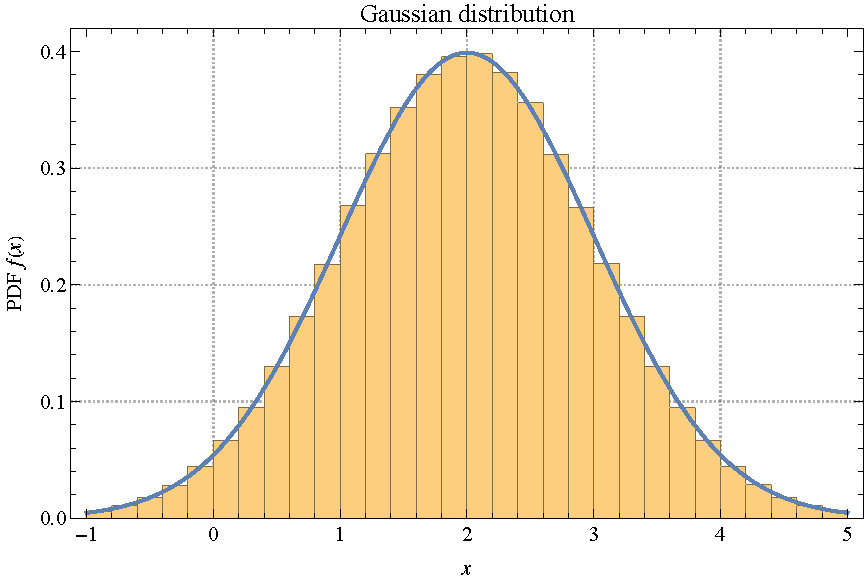
\includegraphics{exercise/change_of_var_Gaussian.pdf}
	\caption[Distribution of $x$ obeying Gaussian distribution.][6pt]{Distribution of $x$ obeying Gaussian distribution.}
	\label{fig:change_of_var_Gaussian}
\end{figure}

\begin{figure}
	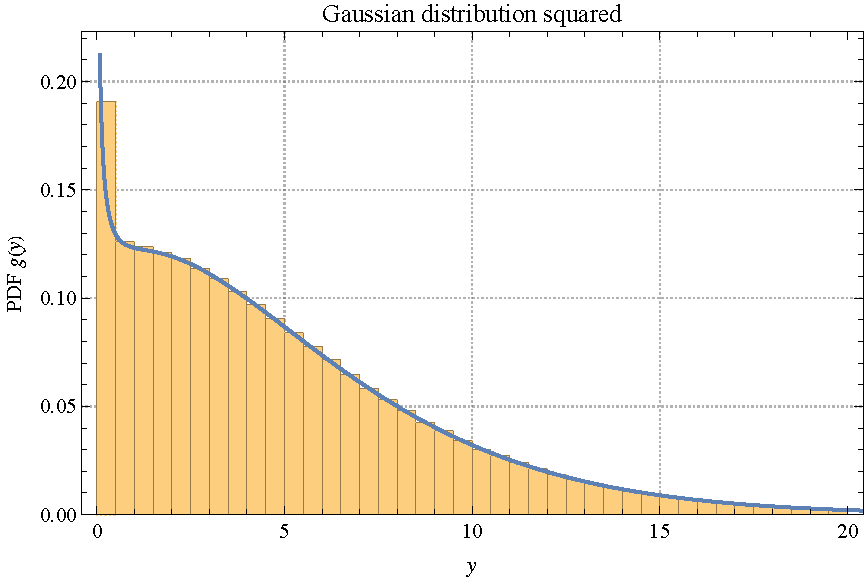
\includegraphics{exercise/change_of_var_Gaussian_squared.pdf}
	\caption[Distribution of $y = x^{2}$ from $x$ obeying Gaussian distribution.][6pt]{Distribution of $y = x^{2}$ from $x$ obeying Gaussian distribution.}
	\label{fig:change_of_var_Gaussian_squared}
\end{figure}

\paragraph{Poisson distribution}\index{Poisson distribution}

\begin{enumerate}
	\item Repeat for $x$ with a Poisson distribution with $\lambda = 3$. (Figure~\ref{fig:change_of_var_Poisson} and~\ref{fig:change_of_var_Poisson_squared})
\end{enumerate}

\begin{figure}
	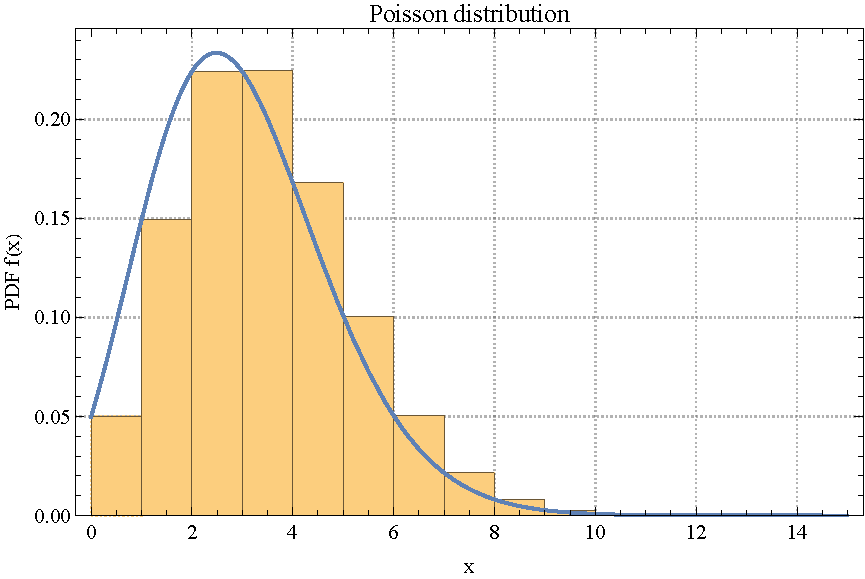
\includegraphics{exercise/change_of_var_Poisson.pdf}
	\caption[Distribution of $x$ obeying Poisson distribution.][6pt]{Distribution of $x$ obeying Poisson distribution.}
	\label{fig:change_of_var_Poisson}
\end{figure}

\begin{figure}
	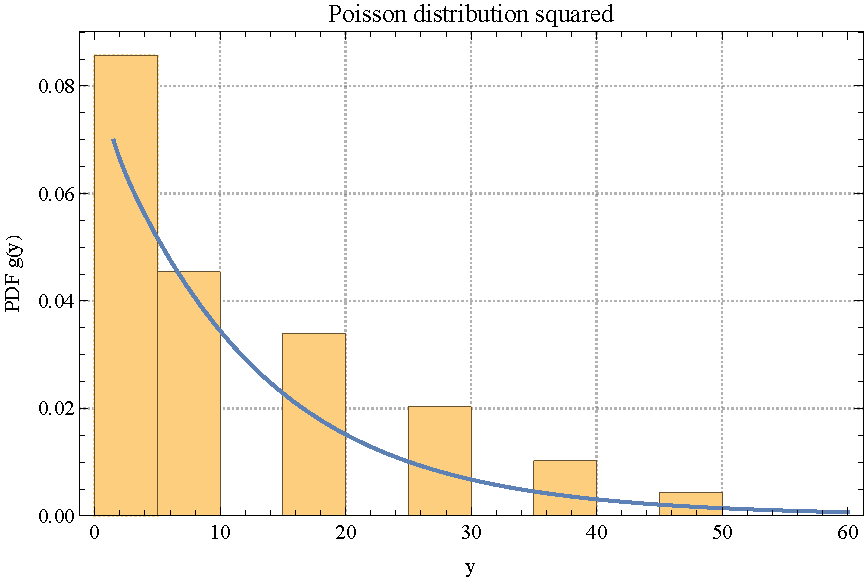
\includegraphics{exercise/change_of_var_Poisson_squared.pdf}
	\caption[Distribution of $y = x^{2}$ from $x$ obeying Poisson distribution.][6pt]{Distribution of $y = x^{2}$ from $x$ obeying Poisson distribution.}
	\label{fig:change_of_var_Poisson_squared}
\end{figure}

($\hookleftarrow$ \ref{subsec:change_of_var})

\newpage

\subsection{Ratio}\index{change of variable!ratio}
\label{exer:change_of_var_ratio}

\begin{enumerate}
	\item Take the variables $x$ and $y$, both Gaussian distributed with $\mu = 0$ and $\sigma = 1$.
	\item Compute the distribution of their ratio analytically and numerically.
\end{enumerate}

\paragraph{Analytical solution}

\begin{description}
	\item Define a change of variable: $u = \frac{x}{y}$, $v = y$.
	\item The joint-PDF\index{joint probability distribution} is:
		$$
		h(u, v) \,\mathrm{d}u \mathrm{d}v = f(x) g(y) \,\mathrm{d}x \mathrm{d}y 
		= f(uv) g(v) \left| \frac{\mathrm{d}(x, y)}{\mathrm{d}(u, v)}\right| \,\mathrm{d}u \mathrm{d}v 
		= f(uv) g(v) v \,\mathrm{d}u \mathrm{d}v
		$$
	\item The PDF\index{marginal distribution} of $u$ is:
		\marginnote[6pt]{This is the special case of Cauchy distribution\index{Cauchy distribution} with $x_{0}=0$ and $\gamma =1$, and is called the standard Cauchy distribution.}
		$$
		p(u) = \int_{-\infty}^{\infty} {f(uv)g(v)v} \,\mathrm{d}v 
		= \int_{0}^{\infty} {f(uv)g(v)v} \,\mathrm{d}v 
		= \frac{1}{\pi (1 + u^{2})}
		$$
\end{description}

\newpage

\paragraph{Numerical solution} (Figure~\ref{fig:change_of_var_ratio})

\begin{figure*}[h]
	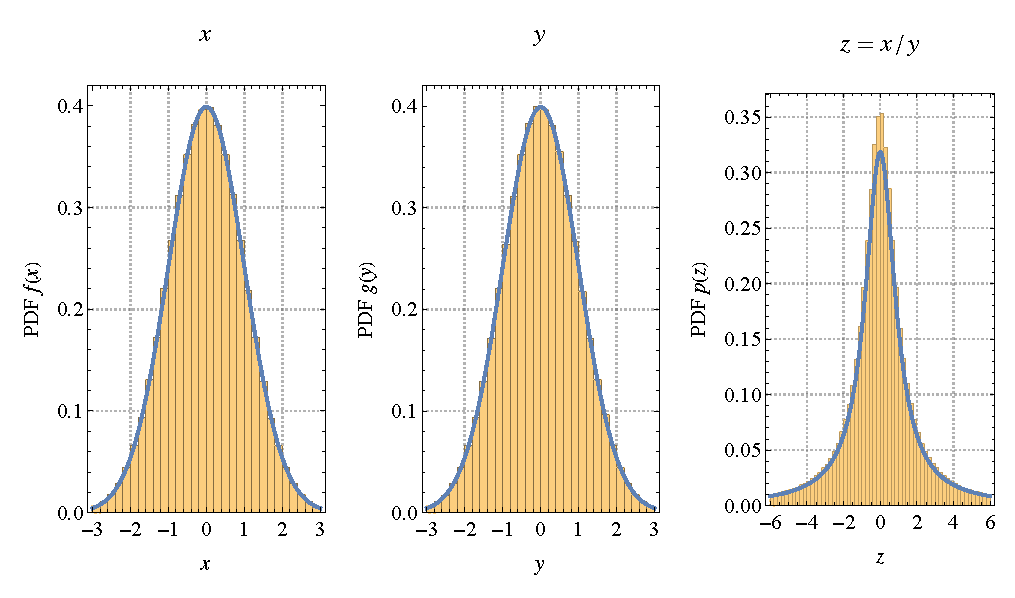
\includegraphics[width=\linewidth]{exercise/change_of_var_ratio.pdf}
	\caption[Distribution of the ratio between $x$ and $y$, both Gaussian distributed.]{Distribution of the ratio between $x$ and $y$, both Gaussian distributed with $\mu = 0$ and $\sigma = 1$.}
	\label{fig:change_of_var_ratio}
\end{figure*}

($\hookleftarrow$ \ref{subsec:prop_of_pseudorandom_number_generator})
